\documentclass[xcolor=svgnames]{beamer}
\usepackage[utf8]{inputenc} % set input encoding (not needed with XeLaTeX)
\mode<presentation> 

%\usetheme{Madrid}

\usepackage{xcolor}

\usepackage[greek,english]{babel}

%\definecolor{maincolor}{RGB}{102, 204, 51}
\definecolor{maincolor}{RGB}{51, 102, 204}
\colorlet{lightermain}{maincolor!35}
\colorlet{darkermain}{maincolor!90!black}

\usetheme{Frankfurt}
%\usecolortheme[named=SeaGreen]{structure}
\useinnertheme{circles}

% \useoutertheme{tree}
% %\usecolortheme[rgb={0.97,0.35,0.04}]{structure}
\usecolortheme[RGB={51, 102, 204}]{structure}

\setbeamercovered{transparent}
\setbeamerfont{block title}{size={}}   
\setbeamertemplate{blocks}[rounded][shadow=true]  
  
\usepackage{verbatim}  
\usepackage{moreverb}
\usepackage{lmodern} 


\usepackage{tikz}
\usetikzlibrary{calc}
\usepackage{gnuplot-lua-tikz}
\usepackage[svgnames]{xcolor}
\usepackage{multicol,multirow}
\usepackage{marvosym}
\usepackage{wasysym}

\newcommand{\comodi}{\textsc{comodi}}
\newcommand{\comoditext}{\textsc{co}unting \textsc{mo}del \textsc{di}fferences}
\newcommand{\grimm}{$\mathcal{G}$\textsc{rimm}}
\newcommand{\grrimm}{$\mathcal{G}$\reflectbox{\textsc{r}}\textsc{rimm}}
\newcommand{\grrimmtext}{$\mathcal{G}$enerating \reflectbox{\textsc{r}}andomized and \textsc{r}elevant \textsc{i}nstances of \textsc{m}eta-\textsc{m}odels}
\newcommand{\grimmtext}{$\mathcal{G}$ene\textsc{r}ating \textsc{i}nstances of \textsc{m}eta-\textsc{m}odels}

\newcommand\un{\includegraphics[scale=0.52]{figs/un.pdf}}
\newcommand\zero{\includegraphics[scale=0.52]{figs/zero.pdf}}

\definecolor{adhal}{RGB}{67,128,54} 

\newcommand\nb[3]{
    \fbox{\bfseries\sffamily\scriptsize#1}
    {\sf\small\textit{\textcolor{#2}{#3}}}
}

\xdefinecolor{DG}{named}{ForestGreen}


\newcommand\green[1]{\textcolor{DG}{#1}}
\newcommand\red[1]{\textcolor{red}{#1}}

\newcommand\add[1]{\nb{Add}{green}{#1}}
\newcommand\urgent[1]{\nb{Add}{red}{#1}}

\newcommand{\letitre}{Tutorial: Create a graphical editor with Eclipse Sirius}

\title{\letitre} 
\author{Adel Ferdjoukh} 
\date{November 2018}  	
  	
%\renewcommand{\inserttotalframenumber}{35}  

%\addtobeamertemplate{footline}{~~-\insertframenumber/\inserttotalframenumber-~\vspace{1mm}} 

\newcommand{\numero}[2]{%
  \begin{tikzpicture}[remember picture, overlay]

    \node[circle,draw] (X21) at ($(0,0)+(0.3,0.2)$) {#2};
    \node[circle,draw] (X22) at ($(X21)+(0.5,0.0)$) {\inserttotalframenumber};
   
  \end{tikzpicture}
} 

\setbeamertemplate{footline}
{
  \vspace{1mm}
  \pgfmathparse{int(\textwidth/\inserttotalframenumber)*\insertframenumber-20}
  \rule{\pgfmathresult pt}{0.2cm}
  \numero{\pgfmathresult}{\insertframenumber}
  \vspace{1mm}
}

%%%%%%%%%%%%%%%%%%%%%%%%%%%%%%%%%%%%%%%%%%%%%%%%%%%%%%%%%
%                                                       %
%    Header                                             %    
%                                                       %
%%%%%%%%%%%%%%%%%%%%%%%%%%%%%%%%%%%%%%%%%%%%%%%%%%%%%%%%%

\newcommand\utopia{\fontfamily{put}\selectfont}
\newcommand\palatino{\fontfamily{pnc}\selectfont}

\newcommand{\header}[4]{%
% #1 Martin Dupont
% #2 other authors
% #3 Title
% #4 Where
  \begin{tikzpicture}[remember picture, overlay]
    % Colored bar on top of the page
    \node [minimum height=2.5cm,fill=darkermain, minimum width=\paperwidth, outer sep=0] (head) at ($(current page.center)-(0,1.6)$) {};
    % Node for the name
        % Address
    \node[anchor=north,below,text=white] (title) at ($(head.north)-(0,0.3)$)  {
      \fontsize{9pt}{7pt}\color{white}
      \utopia #3 \par};

    \node[anchor=base, text=white,below, inner sep=0.25 cm] (name) at (title.south) {%
          \fontsize{9pt}{7pt}\color{white}%
          {\palatino {#1}}
          \fontsize{6pt}{5pt}\color{white} 
          {\palatino #2 \par}
          };

    % Phone/mail/nationality
    \node[anchor=north, text=white] (date) at (name.south)  {\fontsize{7pt}{5pt}\color{white} \utopia #4};

    \node[anchor=north] at ($(date.south)-(0,0.2)$) 
      {
\includegraphics[width=1.05cm]{big.png}~
      
\includegraphics[width=1cm]{TU.png}};

  \end{tikzpicture}
} 


\newcommand{\cg}[1]{\textcolor{gray}{#1}}
\newcommand{\re}[1]{\textcolor{red}{#1}}
\newcommand{\gr}[1]{\textcolor{green}{#1}}
\newcommand{\bl}[1]{\textcolor{blue}{#1}}
\newcommand{\raus}[1]{}

\newcommand{\ra}{$\rightarrow$~}

%\newcommand{\smallblock}[1]{\medskip \rule{0.7cm}{0.07cm} \\ {\large #1} \\ }
\newcommand{\smallblock}[1]{\medskip \textcolor{red}{\rule{0.7cm}{0.07cm}} \\ {\large \sc #1} \\}

\newcounter{step}
\setcounter{step}{0}
\newcommand{\nextstep}{\addtocounter{step}{1}\thestep}

\begin{document}

% %%%%%%%%%%%%%%%%%%%%%%%%%%%%%%%%%%%%
% %                                  %
% %   Page de Azul                   %
% %                                  %
% %%%%%%%%%%%%%%%%%%%%%%%%%%%%%%%%%%%%    
%  \usebackgroundtemplate{
\includegraphics[width=\paperwidth]{azul.png}}  

%  \begin{frame}

%     \thispagestyle{empty}
%     ~

%  \end{frame}

%%%%%%%%%%%%%%%%%%%%%%%%%%%%%%%%%%%%%%%%%%%%%%%%%%%%%%%%%
%                                                       %
%    Page de garde                                      %    
%                                                       %
%%%%%%%%%%%%%%%%%%%%%%%%%%%%%%%%%%%%%%%%%%%%%%%%%%%%%%%%%
\usebackgroundtemplate{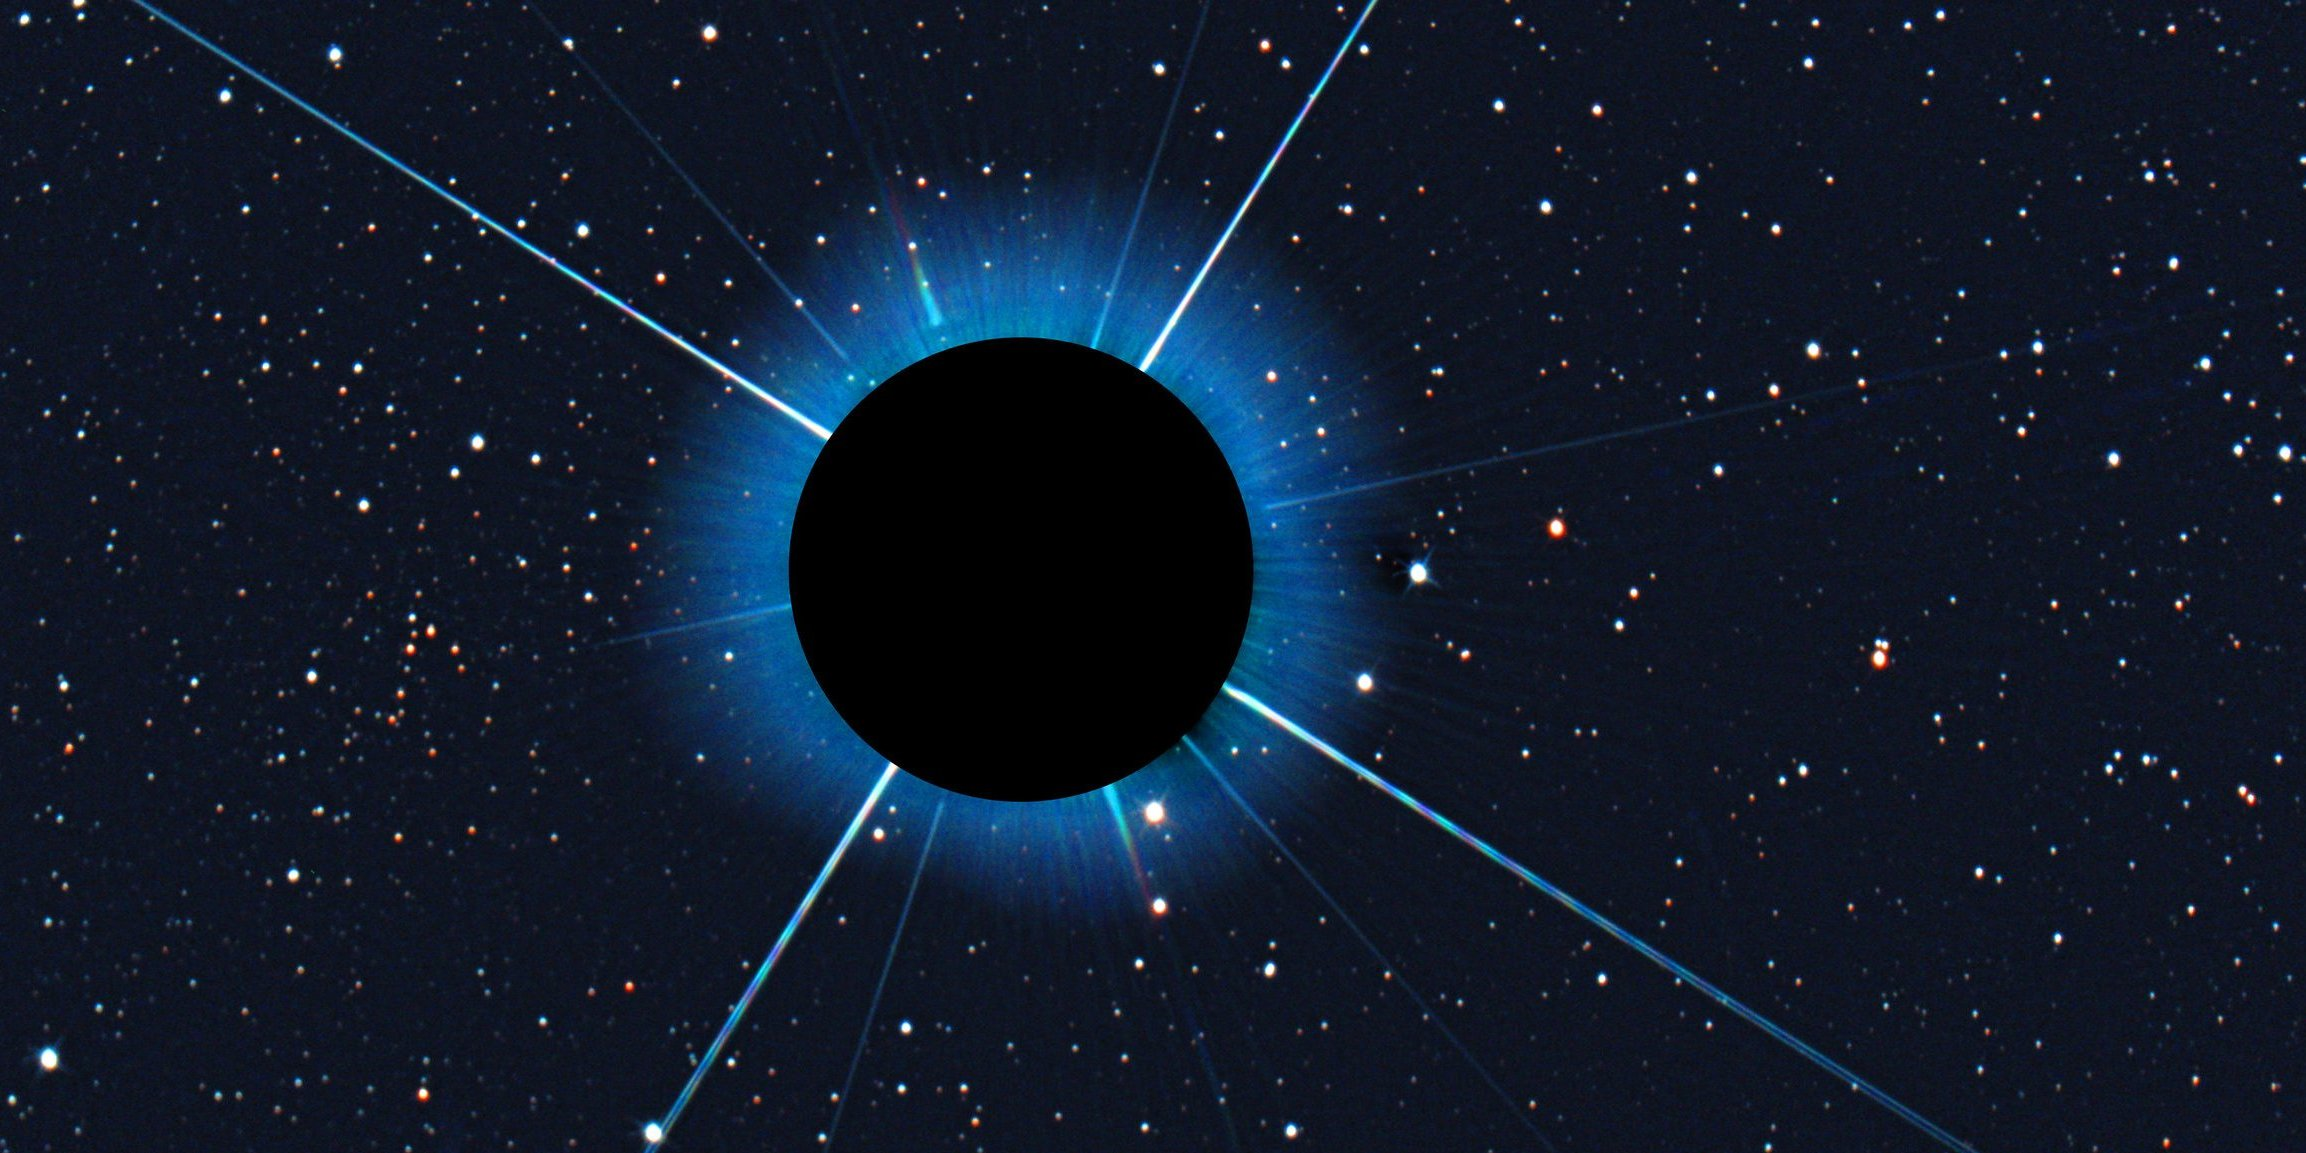
\includegraphics[width=\paperwidth]{sirius.jpg}} 

\begin{frame}
\thispagestyle{empty}
~
\header{Dr. Adel Ferdjoukh}{}{\letitre}{Model Engineering, TU Wien}

\end{frame}

\usebackgroundtemplate{null} 

\begin{frame}{Synopsis}

\tableofcontents[hideallsubsections]

\end{frame}

\section{Create a modelling project}

%%%%
%%%%
%%%%
\begin{frame}{What you need to start this tutorial}

\smallblock{Needed data}

	\begin{enumerate}
		\item Ecore Meta-model (here we use maps.ecore).
		\item Images and icons for elements (given images folder).
		\item Eclipse EMF.
		\item Install Sirius in Eclipse .
	\end{enumerate}

\end{frame}	

%%%%
%%%%
%%%%
\begin{frame}{Create a Modelling project}

\smallblock{step \nextstep : Create an empty modelling project}

	\begin{enumerate}
		\item File \ra New \ra Empty modelling project.
		\item Copy {\it maps.ecore} and {\it images/} into the new project.		
	\end{enumerate}

\end{frame}

%%%%
%%%%
\begin{frame}{Create an EMF generator model}

\smallblock{step \nextstep: Create an EMF Generator Model}

	\begin{enumerate}
		\item maps.ecore Right \ra New \ra EMF Generator Model
	\end{enumerate}

	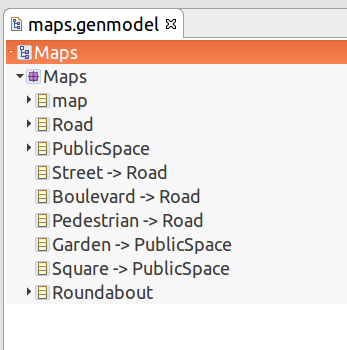
\includegraphics[scale=0.3]{figs/genmodel.png}

\end{frame}


%%%%
%%%%
\begin{frame}{Generate the code of the meta-model}

\smallblock{step \nextstep: Generate the code of the meta-model}

	\begin{enumerate}
		\item in maps.genmodel \ra Maps Right \ra generate all
	\end{enumerate}

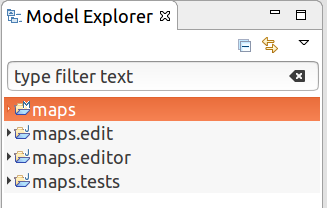
\includegraphics[scale=0.3]{figs/workspace1.png}

\end{frame}

%%%%
%%%%
\begin{frame}{Run maps project as a new Eclipse}

\smallblock{step \nextstep: run as new eclipse application}

	\begin{enumerate}
		\item Run \ra Run as \ra Eclipse Application		
	\end{enumerate}

\end{frame}

%%%%
%%%%
%%%%
\begin{frame}{Create a first instance of the meta-model}

\smallblock{step \nextstep: Create maps Model}

	\begin{enumerate}
		\item In runtime Eclipse: Create a Sirius Project (eg. test)
		\item New \ra maps Model (eg. mapVienna.maps)
		\item Create some elements in mapVienna.maps (new Street, Garden ...)
	\end{enumerate}

	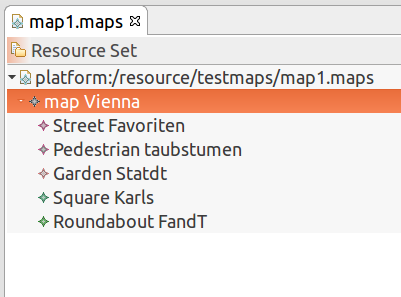
\includegraphics[scale=0.3]{figs/mapVienna1.png}

\end{frame}

\section{Create a Viewpoint Specification project}

%%%%
%%%%
%%%%
\begin{frame}{Create a Viewpoint Specification Project}

\smallblock{step \nextstep: Create a Viewpoint Specification Project}

	\begin{enumerate}
		\item In runtime Eclipse: New \ra Viewpoint Specification Project (eg. maps.design)
		\item a Viewpoint Specification Model is automatically created (maps.odesign)
		\item Rename the root element of .odesign file and set it to maps.
		\item Do the same for the viewpoint element.
	\end{enumerate}

	\centering
	
\includegraphics[scale=0.3]{figs/odesign1.png}

\end{frame}

%%%%
%%%%
%%%%
\begin{frame}{Create a new Diagram Description}

\smallblock{step \nextstep: Create a new Diagram description}

	\begin{enumerate}
		\item In maps.odesign: maps viewpoint right click \ra new representation \ra new Diagram Description
		\item set the properties of the created element: id = map, Domain class= maps.map (the root class of the meta-mode)
		\item Now you can start the creation of you editor
	\end{enumerate}

\end{frame}

%%%%
%%%%
%%%%
\begin{frame}{Test you editor}

\smallblock{step \nextstep: Create a representation}

	\begin{enumerate}
		\item In test project: expand .maps model and right click of root element (use modelling perspective)
		\item New representation \ra other \ra select map
		\item Now you can open map diagram (normally it is empty because no element was created)
	\end{enumerate}

\end{frame}

%%%%
%%%%
%%%%

\section{You graphical editor with Sirius}

%%%%
%%%%
\begin{frame}[allowframebreaks]{Create a first node}

	\smallblock{Create a first node}

	\begin{enumerate}
		\item on Default layer \ra new Diagram Element \ra new Node
		\item set id, domain class and semantic candidate expression of this node.
		\item Create a style for your node (eg. workspace image).
		\item Save and go to the opened diagram. All created streets are now visible.				
	\end{enumerate}	

	\framebreak

	\smallblock{Remark}
	If the Semantic Candidates Expression is not set, then all the streets in you project are selected. To fix that, set: {\bf feature:roads}. Now, only the roads of the current maps model are selected.

	\centering
	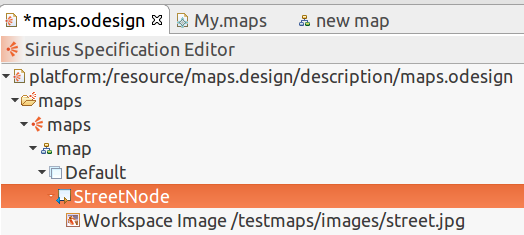
\includegraphics[scale=0.3]{figs/streetNode.png}

\end{frame}

%%%%
%%%%
\begin{frame}[allowframebreaks]{Create a conditional style node}

	Our goal here is to create a conditional style for Boulevard (horizontal or vertical Boulevard). For that we have two different images for Boulevard.

	\begin{enumerate}
		\item Create the Boulevard node
		\item Create a conditional style (set it to [ self.card = maps::cards::East or self.card = maps::cards::West  /])
		\item Create a style for this conditional style
		\item Create a second conditional style
	\end{enumerate}

	\centering
	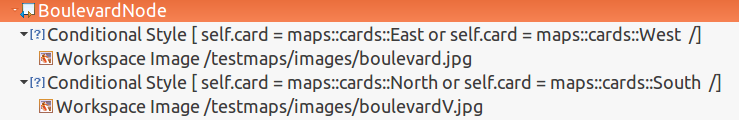
\includegraphics[scale=0.3]{figs/BoulevardNode.png}
	
\end{frame}

%%%%
%%%%
\begin{frame}[allowframebreaks]{Some other examples}

	\smallblock{Remark}
	
	You can find a completed example of a graphical editor created with Sirius (maps.odesign)


	\smallblock{More examples}
	
	In the completed example maps.odesign, you can find the following examples created:

	\begin{enumerate}
		\item Relation based Edge
		\item Palette creation of Node
		\item Palette creation of Relation based Edge
	\end{enumerate}

\end{frame}


\end{document}